\documentclass[12pt, letterpaper, titlepage]{article}
\usepackage[utf8]{inputenc}
\usepackage{geometry}
\usepackage{color,graphicx,overpic} 
\usepackage{fancyhdr}
\usepackage{amsmath,amsthm,amsfonts,amssymb}
\usepackage{mathtools}
\usepackage{hyperref}
\usepackage{multicol}
\usepackage{array}
\usepackage{float}
\usepackage{blindtext}
\usepackage{longtable}
\usepackage{scrextend}
\usepackage[font=small,labelfont=bf]{caption}
\usepackage[framemethod=tikz]{mdframed}
\usepackage{calc}
\usepackage{titlesec}
\usepackage{listings}
\usepackage[normalem]{ulem}
\usepackage{tabularx}
\usepackage{mathrsfs}
\usepackage{bookmark}
\usepackage{setspace}
\usepackage{booktabs}

\mathtoolsset{showonlyrefs}  
\allowdisplaybreaks

\definecolor{mycolor}{rgb}{0, 0, 0}

\geometry{top=2.54cm, left=2.54cm, right=2.54cm, bottom=2.54cm}
\setlength{\headheight}{20pt}
\setlength{\parskip}{0.3cm}
\setlength{\parindent}{1cm}

\pagestyle{fancy}
\fancyhf{}
\rhead{Lora Ma - 1570935}
\lhead{\textit{ECE 322 Assignment 1}}
\rfoot{Page \thepage}

\begin{document} 
\singlespacing

\section{Introduction}
The purpose of this lab was to serve as a practical introduction to rudimentary black-box testing techniques. Although there are an extensive number of black-box testing techniques, in this lab, we were only introduced to generic methods such as dirty testing, error guessing, and partition testing. Black-box testing is testing with no knowledge of the internal structure or implementation details of the program.

\section{Part 1 -- Calculator Program}
\subsection*{Q1}
 The application being tested is a simple calculator that implements a number of standard calculator operations such as addition, subtraction, multiplication,and division. In general, we are trying to write test cases to check if the calculator function as expected. This may involve testing if the buttons are functional, testing character input, testing small/large numbers, testing incorrect syntax, and testing order of operations.

\subsection*{Q2}
We are using dirty testing and error guessing to test the simple calculator. Dirty testing and error guessing usually involves testing out of the box. Sometimes using the tester's previous experience of testing similar products may be helpful. These kinds of tests aim to break the software to show that it does not work. A piece of software must have sufficient exception handling capabilities to survive a significant level of dirty tests. Q4 contains the full list of test cases where the highlighted test cases are the ones with unexpected results. From experience, I believe the following could be reasons for the failures: 
\begin{enumerate}
    \item $2^{150}$ is an extremely large number. The calculator perhaps was not designed to support such large numbers.
    \item It's likely that numbers separated by a space, such as 1 1, simply get concatenated to 11. Because of this, when numbers are encased in brackets (1)(1), it also concatenates them instead of multiplying them.
    \item  When there's a bracket followed by a minus sign, such as $(2^3)-1$ the program may get confused and think that there's two numbers $(2^3)$ and $-1$ with no operation between them. This could be why the output is NaN.
    \item When there's several addition symbols back to back such as $2+++2$, it seems like the program assumes every plus after the first plus is used to describe a positive number. This is why the actual result we got was 4. 
\end{enumerate}

\subsection*{Q3}
The testing methods employed in this section were able to find several errors in the calculator program, but was not able to identify all errors. It is possible that there are many more errors in the program that we were not able to identify. This testing method requires creativity and experience to come up with unconventional test cases and is limited by the tester's creativity. This can be unreliable and may result in lots of unnecessary test cases. 

\subsection*{Q4}
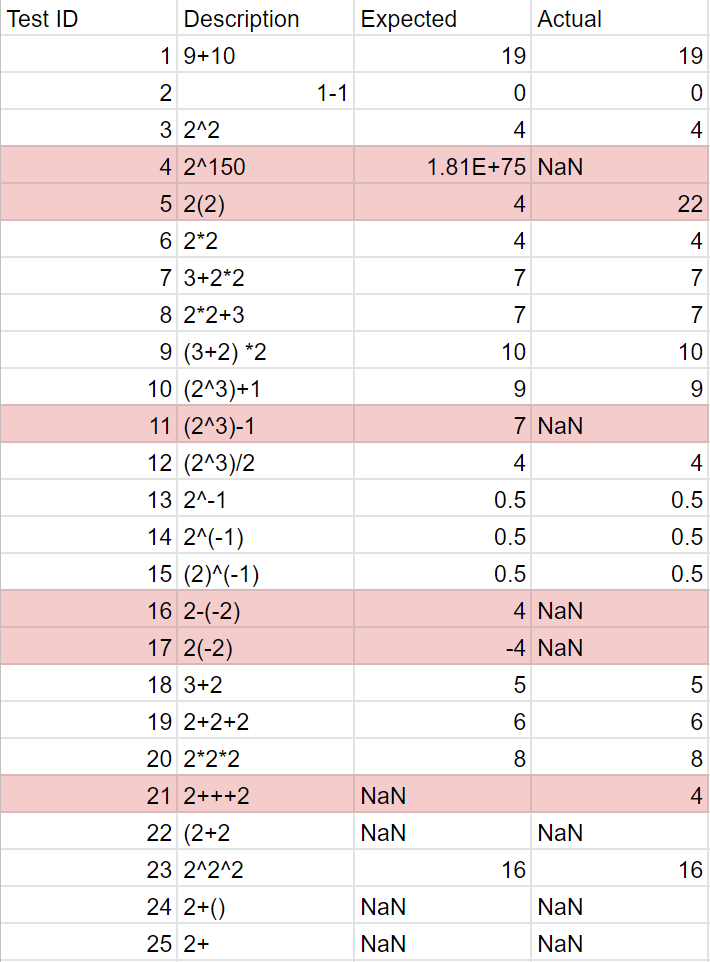
\includegraphics[width=10cm]{table1}

\section{Part 2 -- Triangle Classification Program}
\subsection*{Q1}
The application being tested is a command line triangle classification program. The triangle application reads in three space separated positive integers (a, b, c) representing the length of each side of the triangle, and outputs either the type of triangle (scalene, isosceles, or equilateral) or prints an error message to the console. In this section, we will be using partition testing. In partition testing, we try to categorize test cases into equivalence classes. Through partition testing, we try to cover as many possibilities as possible with as few test cases as possible. This usually results in a lower amount of test cases.

\subsection*{Q2}
Triangle Equivalence Classes
\begin{table}[h]
    \begin{tabular}{|l|l|l|}
    \hline
    Input Condition & Valid Input Class & Invalid Input Class                                            \\ \hline
    \# of input args &
      3 input args &
      \begin{tabular}[c]{@{}l@{}}\textless 3 input args\\ \textgreater 3 input args\end{tabular} \\ \hline
    Type of args    & Positive ints     & \begin{tabular}[c]{@{}l@{}}Neg ints\\ Decimal\\ 0\end{tabular} \\ \hline
    Type of triangle &
      \begin{tabular}[c]{@{}l@{}}Equilateral\\ Isosceles\\ Scalene\end{tabular} &
      \begin{tabular}[c]{@{}l@{}}a + b = c\\ a + b \textless c\end{tabular} \\ \hline
    \end{tabular}
\end{table}

\subsection*{Q3}
In Q5, we can see a list of our test cases. The highlighted test cases are the test cases that had an unexpected outcome. There was one test case that failed our test. This was for the test case where $a = 2, b = 2, c = 4$. We expected the program to output ``ERROR: Not a valid triangle", but it actually said that it was an isosceles triangle. This is likely because the program only checks if $a+b > c$ instead of $a+b \geq c$.

\subsection*{Q4}
The testing methods employed in this section were able to find some important errors in the program. Partition-based testing resulted in having significantly less tests than dirty testing and still was effective in finding the more obvious errors; however, it seems to be less effective at testing unique cases.

\subsection*{Q5}
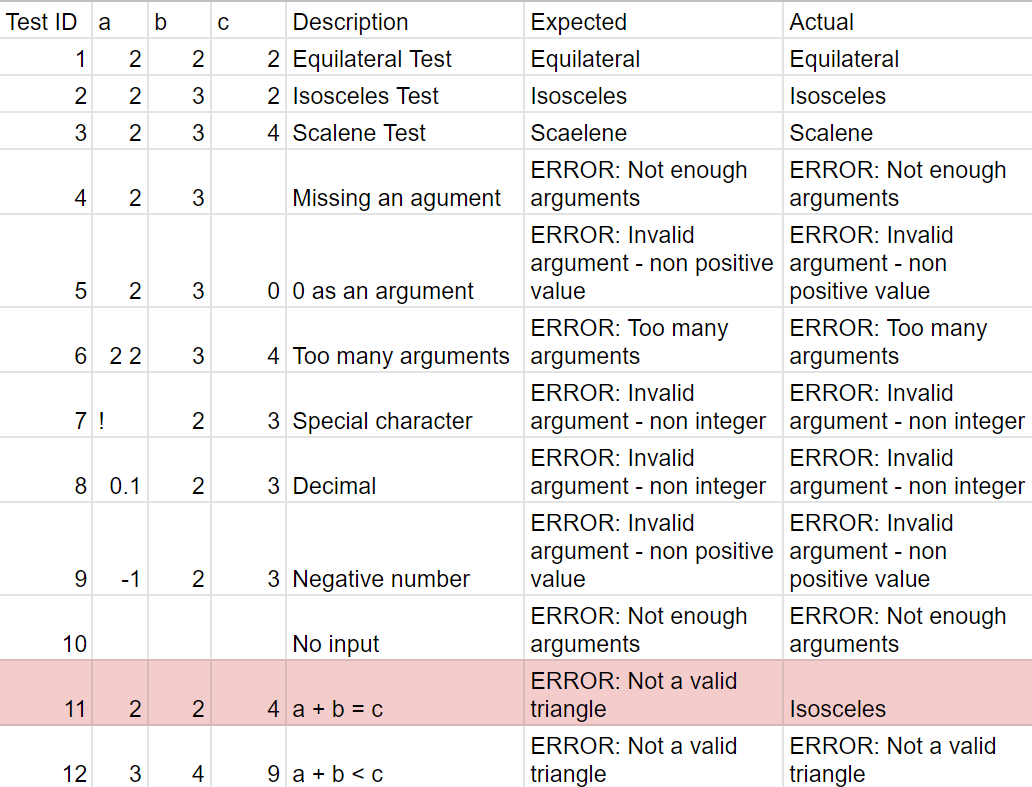
\includegraphics[width=15cm]{table2}

\section{Conclusion}
In this lab, we were introduced to black-box testing. Specifically, dirty testing, error guessing, and partition based testing. We learned that dirty testing and error guessing involves testing every possible input/action a user can perform on the software. It requires testers to be creative and look for unique errors by thinking outside of the box. With more experience in testing similar software, these types of testing may become more effective as the tests are only as good as the creativity of the tester. For partition based testing, we were able to cover as many possibilities as possible with as little test cases as possible, but were unable to test unique cases. In the end, one testing method doesn't seem to be better than the other and the tester should choose the appropriate method for the program they want to test.

\end{document}